\documentclass[pageno]{jpaper}

%replace XXX with the submission number you are given from the ASPLOS submission site.
\newcommand{\asplossubmissionnumber}{XXX}
\newtheorem{theorem}{\bf Theorem}
%\newenvironment{proof}{\par \noindent {\bf Proof: }}{\begin{flushright}
%$\Box$\endflushright}\par \noindent}
\newtheorem{definition}[theorem]{\bf Definition}
\newtheorem{assumption}[theorem]{\bf Assumption}
\newenvironment{proof}{\par \noindent {\bf Proof:}}{\begin{flushright}$\Box$\end{flushright}\par \noindent}
\newtheorem{lemma}{\bf Lemma}
\newtheorem{corollary}[theorem]{\bf Corollary}
\newcommand{\pari}{\hspace{\parindent}}

\usepackage{amsmath}
\usepackage{latexsym}
\usepackage{amssymb}
\usepackage[normalem]{ulem}
\usepackage{upgreek}

\begin{document}

\title{Classifying-based Bias-Global Scheduling Framework\\ for Asymmetric Multicore Processors} 
%Partial Global Scheduling: A Classifying-based Runtime Framework for Asymmetric Multicore Processors}

\date{}
\maketitle

\thispagestyle{empty}

\begin{abstract}

Runtime scheduling is critical for the performance of applications running on asymmetric multicore processors. Global scheduling with preemptions and efficient underlining selection policies can flexibly apply hardware resources to handle multi-thread applications, but suffers heavy overhead from frequent migrations. Useless migrations always caused by the greedy decisions from the scheduler - a current optimal decision may not lead to a better result later.  
Partition-based scheduling framework does well in single-thread applications but loose balancing and causes resource idle for multi-thread applications.  

To address those issues, we come up with the Partial global scheduling - a classifying-based runtime framework. Our theoretical work demonstrates that the proposed partial-global framework do avoid useless migrations against fully global scheduling. Based on this, the classifying-based scheduler can make non-greedy decisions to improve overall system performance.

The experimental results running in GEM5 simulator targeting on ARM big.LITTLE architecture with multiple multi-thread applications from PARSEC, SPLASH2 and mixed with single-thread applications from SPEC2006 suites demonstrate up-to 20\% performance gain from our approach against both the widely used Linux CFS general scheduler and the state-of-the-art WASH schedulers for AMP-specific architecture.

\end{abstract}

\section{Introduction}
\label{itr}
For decades, heterogeneous processors have been verified to be a main trend for both research communities and industrial against traditional multicore processors. More specific, single-ISA asymmetric multicore processors(AMP) provide a new opportunity to further improve system performance with low energy consumption than symmetric multicore processors(SMP).  This advantage is fundamentally achieved by the collaboration of asymmetric hardware support in AMP: High-performance out-of-order big core to improve performance and low-energy in-order little core to save energy.  

Followed by the development of AMPs, improving system performance by efficient OS scheduling targeting specific on this architecture has became a main concern in the literature \cite{mittal2016survey}. Note that the asymmetric hardware resources also make the scheduling space much more complex than before. To demonstrate this complexity and difficulty, we summarise those issues by two critical functions for runtime scheduling:

\begin{itemize}
\item Runtime CPU Selection: This represents the process when a thread is ready to be executed, which CPU will be selected and then put this thread to its associated run-queue. This function can be invoked not only in the beginning when a thread is forked, but also during runtime when a thread is just wake up from sleeping. The asymmetric hardware make this process more complex than SMP as each candidate CPU is different not only by their runtime information (current states, load history), but also from their fundamental computing capacities.  
\item Runtime Thread Selection: This represents the process when a CPU is ready to execute a new task, which thread will be selected right now. This function will be invoked either in the beginning when the hardware is setup or when a CPU finishes it current task or by preemption during runtime. From a global-scheduling\cite{jeff2013big} point of view, the candidate threads are from both this CPU own run-queue and other CPUs run-queue. The asymmetric hardware make this process more complex than SMP as each candidate thread will obtain different speedup from little core to big core. 
\end{itemize}


Multiple efforts from research communities has applied on improving the performance of those two functions separately by considering different critical factors, including core sensitivity \cite{jibaja2016portable,cao2012yin}, bottleneck acceleration \cite{han2018multicore,joao2013utility,joao2012bottleneck,suleman2009accelerating}
and load balancing \cite{kim2018exploring,wang2016rebudget,van2013fairness,van2012scheduling}. To the best of knowledge, we come up with two open problems need to be solved by the research community:

\begin{itemize}
\item[1.] No runtime predicted model  can give wonderful speedup prediction to rank different threads on asymmetric cores. The priority of multiple threads are definitely change during runtime and predicted model trained based on the history or this thread or by a training set cannot guarantee the precise of this output. From a real-system point of view, even no enough performance counters can be recorded during runtime to build up a efficient machine learning model.   
\item[2.] Even the predicted speedup and other runtime factor is accurate,  the runtime selection decision based on the current information is always in greedy. A current sub-optimal decision may lead to a better future scheduling space while the always-on runtime greedy decision prevent this opportunity. 
\end{itemize}
 
To demonstrate the second problem, scheduling a ready thread from a run-queue in big core to be executed in a ready little core can result in an optimal solution from a greedy point of view, or we say a {\it current} optimal solution. But if this thread will only run on the little core for a tidy bit of time and then move back to a big core by preemption when the big core is ready, the overall runtime overhead from additional migrations may totally defeat the benefit from the hard and useless work on the little core. A high level motivating example is shown in Fig \ref{mt}, where $\mathcal{T}$ is a high priority thread which just ranked in the second position under the current running thread on big core's run-queue. By global scheduling, a ready little core will decide to run this high priority thread $\mathcal{T}$ and migrate it from big core's run-queue. While the problem happens if the big core finish its current thread right after the migration issued by the little core, as the big core will decide to run $\mathcal{T}$ and move it back by preemption. Those frequent runtime selections and migrations do lower the performance in this case.
% In our project, each CPU has one unique run queue associated to it.
\begin{figure}
\centering
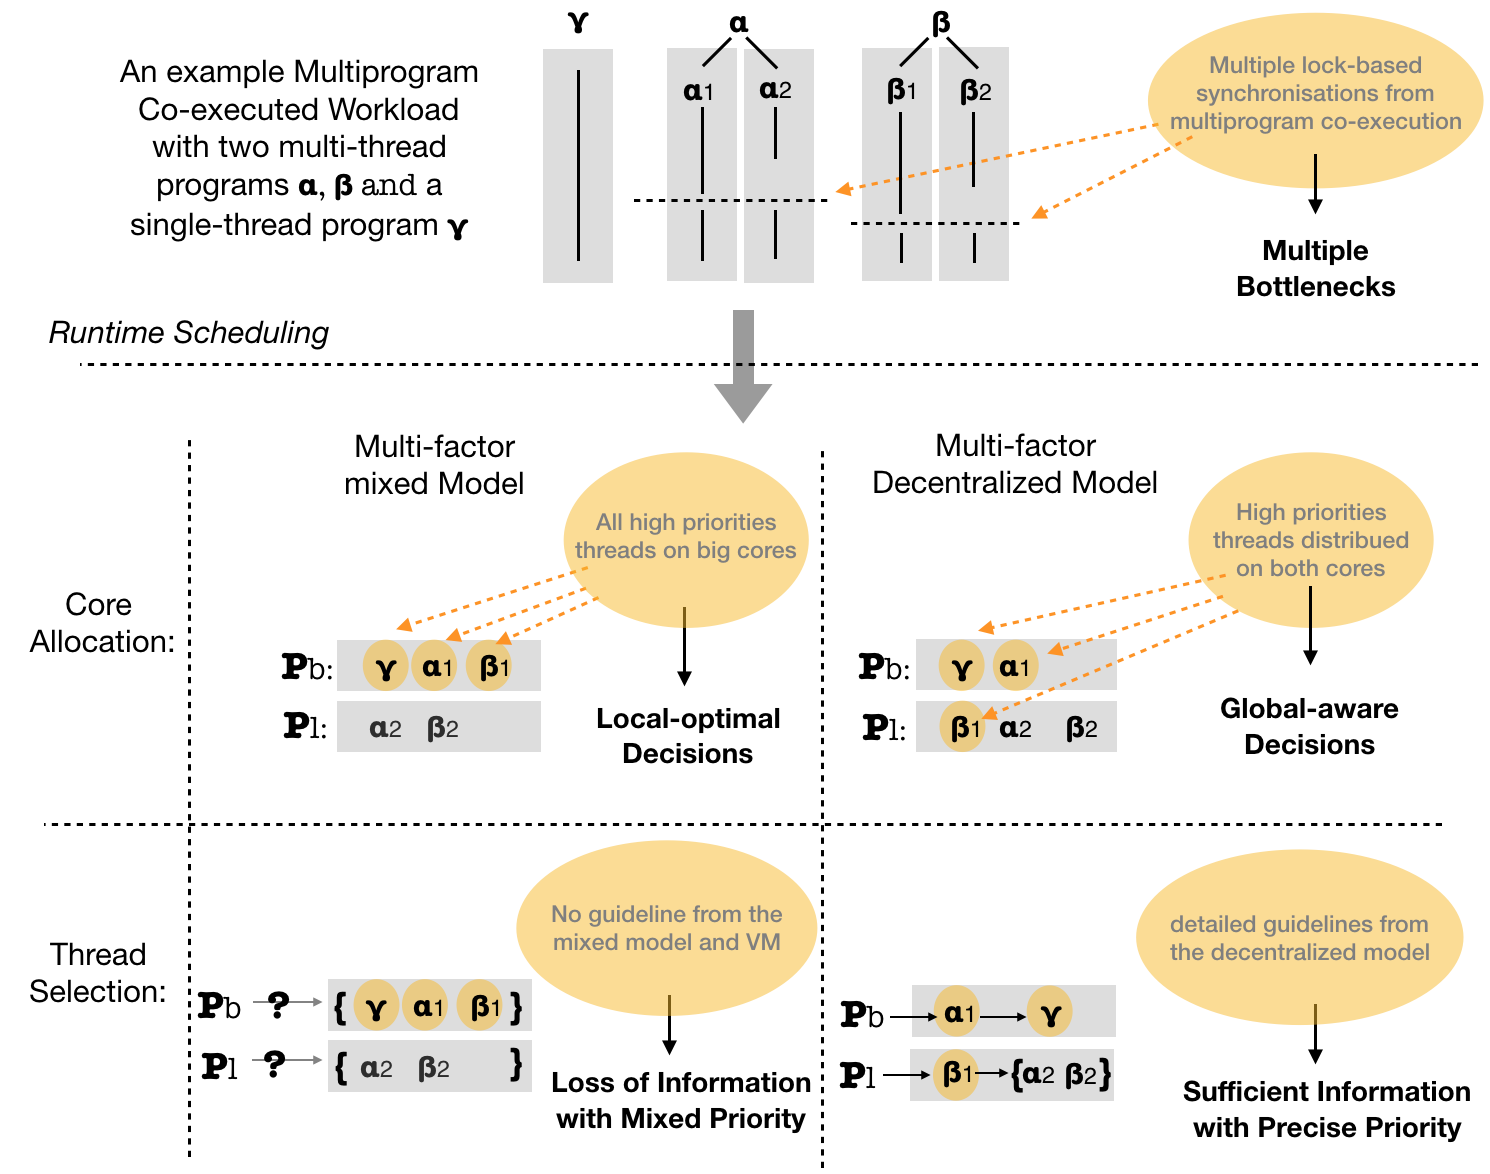
\includegraphics[scale=0.40]{mt.png}
\caption{Motivating Example}
\label{mt}
\end{figure}


Instead of considering the CPU selection and thread selection functions separately and deep in a certain critical factor, we come up with a novel co-designed runtime framework to solve those problems and provide new opportunities for further improvement of overall system performance. In brief, we apply a classifying-based framework which do not aim to rank the priority of different threads precisely and output a deterministic order, but only classify them into three classes based on the hardware heterogeneity: easy class for little core, hard class for big core and medium class for either big or little core. CPU selector then make decisions based on the classifying results hierarchically in fairness - a thread can only select a core in its classified domain. Thread selector then make decisions based on this classifying results in a partial-global way - a core still have the chance to select a thread from another core's run-queue to avoid resource idle, but candidate threads are only from the classified domain. We summarise our main contributions below:
\begin{itemize}[]
\item {\it A partial-global framework which avoids useless runtime overheads established by theoretical analysis.} 
\item {\it A classifying-based scheduler with hierarchical CPU selector and thread selector co-design, which implements the proposed framework and demonstrates high performance for multi-thread applications on AMPs.} 
\end{itemize}
This pioneer work will wake up the potential of further performance gain and encourage following research by applying the runtime classifying framework with cpu allocator and thread scheduler co-design. With the potential of more efficient machine learning based speedup model, the classifier will make more smart decisions.  

The remainder of this paper is presented as follows: Section II describes the background and related work which includes a  description of efforts on different critical factors for runtime scheduling on AMPs. Section III discusses our classifying-based runtime framework which includes a description of the classifier, the co-designed CPU selector and thread selector. Our experimental design and results analysis are given in section IV. 

\section{Motivation}

Consider we need to compute a formulation below using an asymmetric multicore processor with one big core and one LITTLE core:
$$ \sum^{n}_{i=1} a_i + (\sum^{n-1}_{i=1} a_i)^2 + \sum^{n/5}_{j=1} b_j$$

It is easy to say that an optimal way to compute it on the two-core processor is by using three-thread parallel programming: 

\begin{itemize}
\item $thread\ \mathcal{T}_1: \sum^{n}_{i=1} a_i$
\item $thread\ \mathcal{T}_2: \sum^{n/5}_{j=1} b_j$
\item $thread\ \mathcal{T}_3: (\sum^{n-1}_{i=1} a_i)^2$
\end{itemize}

Initially, $\mathcal{T}_1$ and $\mathcal{T}_2$ will run in parallel on the big core and LITTLE core, while $\mathcal{T}_3$ will be in the runqueue of the big core. Then the LITTLE core will finish his job on $\mathcal{T}_2$ first as it has only 20\% computation to do against $\mathcal{T}_1$ on the big core. This means the LITTLE will be idle and ready to execute new job. After the big core compute $\sum^{n-1}_{i=1} a_i$, the thread $\mathcal{T}_3$ become ready to be executed.

In the global scheduling framework, $\mathcal{T}_3$ will be migrated to the LITTLE core and proposed to execute on there as this core is idle. But right after a tiny bit of time, the big core finishes $\mathcal{T}_1$ as only one adding computation remain and by preemption, $\mathcal{T}_3$ will be migrated back to the big core. In fact, this leads to useless migrations - the thread $\mathcal{T}_3$ can run better if it was always on the big core's runqueue without ever migrated to the LITTLE core.

\section{Background and Related Work}
\label{rw}

\subsection{Bottleneck Identification and Acceleration}
Bottleneck can be defined as any code segment which threads contend. It is critical for performance of multicore systems on parallel executions: Like a barrier where multiple threads need to reach a synchronisation point before others can make new progress. Other bottlenecks are such as critical sections of multi-thread programs and pipeline stages. Failure to accelerate bottleneck can lead to reduce or even stop speedup which could bee expected from parallel executions on multicores. 

An efficient Bottleneck Identification and Scheduling (BIS) approach on AMPs was presented in \cite{joao2012bottleneck}. In addition of their previous efforts \cite{suleman2009accelerating} which can only accelerate one bottleneck at a time on single big core systems, BIS can identify which bottlenecks are most critical at any given time and accelerate them accordingly on big cores. The key idea is to measure the number of cycles spent by each thread when waiting for bottlenecks and then rank and accelerate those bottlenecks based on those values. It is mainly composed by twofolds:

\begin{itemize}
\item[1.] Bottleneck Identification: A bottleneck table (BA) is implemented in which each entry corresponds to a bottleneck and includes a thread waiting cycles field (WCT) to track this information. WCT value is computed by aggregating the number of threads who are waiting on this bottleneck. The critical bottlenecks are then identified by BA with $N$ highest WCT values where $N$ is based on the number of big cores in the system.
\item[2.] Bottleneck Acceleration: To decide whether a bottleneck should be accelerated by big cores, an acceleration index table (AIT) is created associated with each small core. The small cores send bottleneck execution requests based on the information from AIT and those requests are then enqueued in a scheduling buffer (SB) in big cores. SB is actually a priority queue which always run the oldest instance with highest WCT value. To avoid false serialisation and resource starvation, SB also implement an request abort function which will let the big core send back a bottleneck to small cores if this bottleneck does not have the highest WCT value and is ready to run on small cores.
\end{itemize}
Based on the core function from BIS, following approach has been developed in the same track, such as using a utility function to make more efficient bottleneck identification in \cite{joao2013utility} and designing mix-critical level to rank the threads more precisely in \cite{han2018multicore}. 


\subsection{Fairness and Load balancing}
Fairness, or guaranteeing all threads make equal progress is another critical factor of scheduling on heterogeneous multicore processors, especially when targeting on multi-thread workloads with barrier-synchronisation and multi-program workloads with quality-of-service (QoS) constraints.

Two fairness-aware scheduling methods are presented in \cite{van2013fairness}. 
\begin{itemize}
\item[1.] The first one is called $equal$-$time$ scheduling. It trivially keeps each thread to run on each type of cores in same amount of time slices and implemented by Round-robin or random selection of a thread which currently on small core to schedule on big core next. But it cannot imply truly fairness if threads experience different slowdown or speedup from different cores. 
\item[2.] A more advantage approach to handle this fact in their paper is called $equal$-$progress$ scheduling which guarantee each thread reach the equal progress on heterogeneous cores.  The key challenge of this approach is to estimate a big-versus-small-core scaling factor for all threads and then it can be used to compute the slowdown between running on heterogeneous cores and big cores in isolation.  There are three methods provided to obtain this factor: (1) sampling-based method which compute this factor during a sample phase as the ratio between CPI on different cores and then apply on symbiosis phase; (2) history-based method which is similar with the sampling way but records historical CPI values and continuously adjust the ratio; (3) model-based method which use a performance impact estimation (PIE) \cite{van2012scheduling} analytical model to estimate this factor with hardware support.
\end{itemize}
They also mentioned a $guaranteed$-$fairness$ approach based on their scheduler when system throughput need to be concern. A threshold of fairness can be setup and the scheduler will defers to a throughput-optimisation policy after this threshold reached. Overall, fairness-aware scheduler achieve 14\% performance gain on homogeneous multi-thread workloads and 32\% performance gain on heterogeneous multi-thread workloads on average against other schedulers. 

Note that the well-known Linux scheduler is also fairness-oriented which is based on complete fairness scheduling (CFS) \cite{li2009efficient}. Focusing on fairness and designing more efficient fairness-oriented metric functions or market-based metrics is always a main trend in the research community, more work are presented during recent years such as Uniformity \cite{kim2018exploring} and ReBudget\cite{wang2016rebudget}.

\subsection{Heterogeneous Core Sensitivity}
WASH \cite{jibaja2016portable} is the most state-of-the-art scheduler which provides a novel AMP-aware runtime environment which use dynamically analysis to classify application, identify bottleneck and prioritises threads based on single-ISA. It is the first work who can optimise critical path, core sensitivity, priorities and load balancing simultaneously. 

Compared with their previous statical $yin$ and $yang$ based scheduler \cite{cao2012yin} which always bind threads based on static classification, WASH algorithm dynamically and periodically use runtime information about core sensitivity, thread sensitivity and workload to schedule threads. The scheduler starts with scheduling application threads on big cores and VM threads on small cores, and then dynamically classify (scalable or not), prioritise and migrate threads guided by the runtime information.

They implement two models to record and provide those information.
\begin{itemize}
\item[1.] One is named a dynamic bottleneck analysis. The core function is to accelerate threads which hold contended locks by computing an ratio between the time this tread waits for another thread to release a lock and the total execution time of it so far. To prioritise among those threads, it select the one who make others wait the longest to big cores.
\item[2.] The second is a core sensitive predictor. It uses linear regression and Principal Component Analysis to learn most significant performance counters with corresponding weight. The selected counters include such as INSTRCUTIONS\_RETIRED and  L1D\_ALL\_REF:ANY for Intel processors and RETIRED\_UOPS and CPU\_CLK\_UNHALTED for AMD cores. Those counters can then be used to compute the speedup if we schedule a thread on big cores than on small cores. In detail, it involves two relative ranking function. The $ExecRank$ is an adjusted priority which shows how much performance gain can be achieved if the thread is on big cores by accumulating on retired instructions. The $LockRank$ is to show the bottleneck level based on the amount of time other threads have been waiting for it. 
\end{itemize}
Overall, WASH report a up-to 20\% performance gain and 9\% energy save against prior work on heterogeneous multicore AMD cores in different configurations. 




\section{Theoretical Analysis on Scheduling Frameworks}
Consider the multi-thread scheduling problem on AMPs, the main object of improving overall performance is represented by reducing the geometric mean of total life time (from its forked until its dead) of all threads. In another word, we want to reduce the life time of each application thread in the multi-thread workloads.

\subsection{Basic terms}
Now we formularise the problem. For a certain thread $\mathcal{T}$, first we have those basic terms below:
\begin{itemize}
\item[$t$:] the actual life time of  $\mathcal{T}$.
\item[$t_l$:] the actual execution time of $\mathcal{T}$ on little cores.
\item[$t_b$:] the actual execution time of $\mathcal{T}$ on big cores.
\item[$t_o$:] the total interruption time of $\mathcal{T}$ during its life.
\item[$T_l$:] the total execution/life time of $\mathcal{T}$ if run on a little core without any interruption.
\item[$T_b$:] the total execution/life time of $\mathcal{T}$ if run on a big core without any interruption.
\item[$\upmu$:] the relative speedup of $\mathcal{T}$ from little core to big core.
\end{itemize}
Based on those terms, we obtain the two basic definitions:
\begin{definition} $t = t_l + t_b + t_o$
\end{definition}

\begin{definition} $\upmu = \frac{T_l}{T_b}$
\end{definition}

Then the main object is to make $t$ as lower as possible. The lower of resulting $t$, the more efficient of a given scheduling framework. 

\subsection{Scheduling frameworks}
Followed by we present the three scheduling frameworks by how will they handle the thread $\mathcal{T}$:
\begin{itemize}
\item {\it Global Scheduling:} $\mathcal{T}$ can be scheduled in either big core or little core and can be migrated between different types of cores during its life. We use $t_1$ to represent the actual life time of $\mathcal{T}$ under this framework. 
\item {\it Partition-based Scheduling:} $\mathcal{T}$ can only be scheduled in either a big core or a little core and can not be migrated to a different core during its life. We use $t_2$ to represent the actual life time of $\mathcal{T}$ under this framework. 
\item{\it Partial-global Scheduling:} Threads are been classified during runtime into three classes ($hard$, $easy$, $medium$)\footnote{For easy illustration, we assume that  $\mathcal{T}$ is in hard class in this document.} based on its predicted $\upmu$ and other performance factors. $\mathcal{T}$ can only be scheduled into big cores and be migrated within this type of cores during its life if it is classified as in the $hard$ class. We use $t_3$ to represent the actual life time of $\mathcal{T}$ under this framework. 
\end{itemize}

Before we can formularise and define the actual life time of thread $\mathcal{T}$ based on different frameworks, there are several more terms we need to give as below:

\begin{itemize}
\item[$t_m$:] the total migration overhead of $\mathcal{T}$ based on global scheduling framework during its life.
\item[$t'_m$:] the total migration overhead of $\mathcal{T}$ based on partial-global scheduling framework during its life.
\item[$t_p$:] the total time when no any big core can execute $\mathcal{T}$ during its life.
\item[$t'_p$:] the total time when a certain big core can not execute $\mathcal{T}$ during its life.
\item[$t_k$:] the total time when $\mathcal{T}$ is blocked by other threads.
\end{itemize}

Now we can begin to define the actual life time of thread $\mathcal{T}$ based on different frameworks.
\subsubsection{Global Scheduling $t_1$:}
By applying global scheduling framework, we have:
$$ t_b = T_b - t_p;\ t_l = \upmu t_p;\ t_o = t_m + t_k $$
then we can formularise the actual life time  ($t_1$) of $\mathcal{T}$ under this framework as following:
\begin{definition}\label{d1} $$  t_1 =  t_b + t_l + t_o = (T_b - t_p) + \upmu t_p + t_m + t_k $$
\end{definition}

\subsubsection{Partition-based Scheduling $t_2$:}
By applying partition-based scheduling framework, we have:
$$ t_b = T_b;\ t_l = 0 ;\ t_o = t'_p + t_k $$
then we can formularise the actual life time ($t_2$) of $\mathcal{T}$ under this framework as following:
\begin{definition}\label{d2} $$  t_2 =  t_b + t_l + t_o = T_b  + t'_p + t_k $$
\end{definition}

\subsubsection{Partial-global Scheduling $t_3$:}
By applying partial-global scheduling framework, we have:
$$ t_b = T_b;\ t_l = 0;\ t_o = t_p + t'_m + t_k $$
then we can formularise the actual life time ($t_3$) of $\mathcal{T}$ under this framework as following:
\begin{definition}\label{d3} $$  t_3 =  t_b + t_l + t_o = T_b + t_p + t'_m + t_k $$
\end{definition}

\subsubsection{Basic Assumption:}
To make those frameworks act different on thread $\mathcal{T}$, we make the assumption below: 

\begin{assumption} \label{a1} $t_p > 0\ \&\&\ t'_p >0$
\end{assumption}

Note that if $t_p = 0$ and $t'_p = 0$, then all three frameworks will keep to run $\mathcal{T}$ on a certain big core and then $t = T_b$

\subsection{New Theorems}
Before we can compare the performance of different frameworks by analysis on the actual life time of thread $\mathcal{T}$, there are two basic lemmas we should claim: 

\begin{lemma} \label{l1}The total migration overhead in global scheduling framework is not less than in partial-global scheduling: $$t_m \geq t'_m$$
\end{lemma}

\begin{proof} Note that $t_m$ contains the migrations between either big and little cores or within multiple big cores. $t'_m$ only contains the migrations within multiple big cores. Thus, the total times of issuing migrations in the first case must be more than or equal to the second case.
\end{proof}


\begin{lemma}\label{l2} The total time when a certain big core can not execute $\mathcal{T}$ is not less than the total time when no any big cores can execute $\mathcal{T}$: $$t'_p \geq t_p$$
\end{lemma}

\begin{proof} This lemma is trivial as we have at least one big core in the hardware configuration.
\end{proof}

Now we can claim our theorems about the performance and efficiency on different scheduling frameworks:
\begin{theorem}  \label{t1}  Partial-global scheduling is more efficient than global scheduling on thread $\mathcal{T}$ ($t_3 < t_1$) if and only if $\upmu > (2-\frac{t_m - t'_m}{t_p})$
\end{theorem} 

\begin{proof} 
First, we proof that $t_3 < t_1 \mapsto  \upmu > (2-\frac{t_m - t'_m}{t_p})$:\\ Given $t_3 < t_1$, we first apply definition \ref{d1} and \ref{d3} and then obtain: $$ T_b + t_p + t'_m + t_k < (T_b - t_p) + \upmu t_p + t_m + t_k$$ which is equal to: $$ (2 - \upmu) t_p < t_m - t'_m$$ Based on the assumption \ref{a1}, we know that: $t_p > 0$. Then we obtain: $$ 2 - \upmu < \frac{t_m - t'_m}{t_p}$$ which is equal to the target: $$  \upmu > (2-\frac{t_m - t'_m}{t_p}) $$ The process of verifying $ \upmu > (2-\frac{t_m - t'_m}{t_p}) \mapsto t_3 < t_1$ is similar.
\end{proof}

Note that this theorem only shows the underlining relationships between the efficiency of the two given frameworks and multiple un-predictable runtime factors. The corollary from this theorem shown below demonstrates when partial-global scheduling will do better on $\mathcal{T}$ only related to the value of its relative speedup:

\begin{corollary} \label{c1} Partial-global scheduling is more efficient than global scheduling on thread $\mathcal{T}$ if its relative speedup is greater than 2:
$$\upmu > 2 \mapsto t_3 < t_1  $$
\end{corollary}

\begin{proof}
By applying the lemma \ref{l1} above, we obtain: $$ t_m - t'_m \geq 0$$ Note the assumption \ref{a1}, we have $t_p > 0$. Then we have: $$ \frac{t_m - t'_m}{t_p} \geq 0$$ which leads to: $$2 \geq 2 - \frac{t_m - t'_m}{t_p}$$ Given that $\upmu > 2$, we obtain: $$\upmu > (2-\frac{t_m - t'_m}{t_p}) $$ By applying the theorem \ref{t1}, we finish our verification: $$\upmu > 2 \mapsto t_3 < t_1  $$
\end{proof}

This corollary does provide a strong theoretical support for the partial-global scheduling against global scheduling. It shows the partial-global scheduling will definitely do better for $hard$ thread whose relative speedup if greater than 2 whatever its un-predictable runtime factors.

\begin{theorem}  \label{t2}  Partial-global scheduling is more efficient than partition-based scheduling on thread $\mathcal{T}$ if and only if $(t'_p - t_p) > t'_m$
\end{theorem} 

\begin{proof} 
This theorem can be trivially verified by applying the definition \ref{d2} and \ref{d3} directly.
\end{proof}
Note that instead of the corollary \ref{c1} above, this theorem does confirm that the efficiency between those two frameworks are heavily influenced by the three un-predictable runtime factors: $t'_p,\ t_p,\ t'_m$. We cannot easily say which framework will theoretically do better for a $hard$ thread based on this theorem directly. While in practice,  the additional benefits from multiple big cores ($(t'_p - t_p)$) will always overcome the overhead from inter-big-core cluster migrations based on the increase number of big cores and the fact that multiple big cores are usually in one physical cluster. 

On the other hand, for threads which are partitioned into a little core in the partition-based scheduling, the partial-global scheduling do give them a chance to be accelerated on big core. The proposed partial-global scheduling handles those $not$ $hard$ threads similar with the global scheduling with preemption - those threads may also be accelerated on big cores but with a low priority. The only difference is the partial-global scheduling will prefer to allocate the $easy$ class threads into the run-queues of little cores. 






\section{Classifying-based Runtime Design}
\subsection{Runtime Classifier}
Motivated by the state-of-the-art approaches, our runtime classifier consider two critical factors (bottleneck level, speedup level) of threads to classify them. This classifier is invoked periodically during runtime to re-classify the ready threads. Instead of a deterministic heuristic-based approach, it only output one of three possible classes targeting on AMPs and do not further rank threads in each class. Based on the two-type heterogeneous hardware resources,  we list the three possible classes below:
\begin{itemize}
\item[1.] $Easy$ class: a thread obtains low levels from both the bottleneck factor and speedup factor. It should be better to run on little cores to avoid resource wasting and have very low priority for big cores.
\item[2.] $Hard$ class: a thread obtains high levels from both the bottleneck factor and speedup factor. It should be better to run on big cores to accelerate as soon as possible and cannot to be selected by little cores during runtime to avoid useless migrations.
\item[3.] $Medium$ class: the remaining threads which are difficult to determine whether its more suited on big core or little core. Instead of wasting computational resources to give them a non-precisely decision, we put them to the medium class and enjoy a same priority to run either in big core and little core. 
\end{itemize}

Note that (1) the fairness factor is considered by how the classifier is applied on CPU and thread selection instead of inside the designing of classifier; (2) This work is not focusing on developing either a high-efficient novel bottleneck identifier or a high-accurate speedup predictor, so we just equip two common state-of-the-art approaches to handle those two factors in our classifier: 

\subsubsection{Bottleneck Factor}
The bottleneck level in our classifier is mainly recommended by a block\_total performance counter. This counter associates on each thread and records the total amount of time that other threads are been contended by this thread during runtime. The higher value of this counter, the higher bottleneck level this thread will obtain. There is also a relative lower-bound of each thread to reach the bottleneck level. In another word, this bounding value will increase during runtime based on the progress of the programs. 


\subsubsection{Speedup Factor}
We involved a state-of-the-art common approach to include the speedup factor in our runtime classifier. It is based on the common principle that a thread run well in one kind of core will also run well in the future in such core. The machine learning based predicted speedup model is trained offline while applied online. 

First, we run a training set of benchmarks on both full big cores and full LITTLE cores configurations separately, and then record the relative speedup of each thread. Principle Component Analysis (PCA) is applied to select several most critical features (performance counters) for data pre-processing. The list of those features with their relative importance is shown in table \ref{}. Linear regression is then applied to build the linear predicted speedup model based on the selected performance counters. The linear speedup model is formulated as following:
$$ $$
Finally, the speedup model input to the runtime classifier as a critical factor. The classifier is invoked periodically during runtime after a certain time internal. It traverses all ready threads each time and re-classify them into the three targeting classes based on the above two factors. The pseudo-code of this classifier is shown in Algorithm \ref{}. 


\subsection{Hierarchical Round-robin CPU Selector}
Hierarchical round robin processor allocation: Instead of trying hard to design more precisely predicted model either online or offline, we consider an alternative approach by only roughly classify the threads without even rank them. The threads are classified into only three classes: hard, easy and middimim.  The hard threads will only be allocated to big cores while the easy threads will only be allocated to little cores. The middimim threads may either be allocated to big or little cores. We propose three corresponding round robin counters to achieve fairness allocation. The counter for the middimim class is shared value with the other two counters to avoid accumulated allocation from different robins. 

We just apply and update from state-of-the-art bottleneck thread detection methods (such as just based on total number of instructions) to classify the threads, the current work do not focus on designing novel classifier. The total number of hard and easy threads should be less than the number of cores in big and little cluster, separately.


\subsection{Partial-global Thread Selector}
Partial global task selection: The basic method of our runtime task selection is built on global scheduling - each CPU can select a task from others runqueue to achieve high-efficiency. This selection function is triggered by multiple migration technologies as applied in ARM global scheduler. The underlining selection method is based on weighted random number generator (rng) instead of a specific heuristic-based ranking. We add constraints and backtrack to provide the opportunity of making smart decision instead of the greedy decisions - For big cores, if it selects a thread in easy class, we re-run the weighted rng once to find a new result  - instead of having to run the selected task, we let the big core keeps idle or say take a break if the selected task is still in easy class. Similar for little cores - a little core will relax instead of running a hard task after the weighted rng run twice. 

We do not claim that this randomisation-involved approach would definitely results in smart decision, but it does will provide the opportunity to make those kind of decisions. 


\section{Experiments}
\label{ep}

\subsection{Experimental Setup}
The experiments is using GEM5 \cite{binkert2011gem5} simulator. The hardware setup contains 2 big cores and 2 LITTLE cores to simulate a Asymmetric Multicore Processor.


\subsection{Benchmarks}
The benchmarks we applied are from PARSEC 3.0\cite{bienia2008parsec} suites and SPEC2006\cite{henning2006spec}. We select and combine several benchmarks together to build multiple mixed-multi-benchmark workloads.

\subsection{Experimental Metrics}
As a common approach in the literature, we use the geometric mean of execution time of each application thread in a workload combination to represent the system performance, which is also the basic value to compute the more formal $Speedup$\cite{joao2013utility} metric.

\subsection{Experimental Results}

\subsubsection{Results on multiple multi-thread benchmarks workloads}

\subsubsection{Results on mixed multi-thread and single-thread benchmarks workloads}

\section{Conclusion}




%\paragraph{Highlights ({\bf note the following})}:
%\begin{itemize}
%\item Paper must be submitted in printable PDF format.
%\end{itemize}
%\paragraph{Paper evaluation objectives}:


\section{Paper Preparation Instructions}

\subsection{Paper Formatting}

Papers must be submitted in printable PDF format and should contain a
{\bf maximum of 11 pages} of single-spaced two-column text, including any
appendixes, but {\bf not
  including references}.  You may include any number of pages for
references, but see below for more instructions.  If you are using
\LaTeX~\cite{lamport94} to typeset your paper, then we suggest that
you use the template here:
\href{https://asplos-conference.org/wp-content/uploads/2018/06/asplos19-latex-template.tar.gz}{\LaTeX~Template}.
(\href{https://asplos-conference.org/wp-content/uploads/2018/06/asplos19-template.pdf}{This
  document} was prepared with that template.)  If you use a different
software package to typeset your paper, then please adhere to the
guidelines given in Table~\ref{table:formatting}.\footnote{One
  exception is that authors may use the SIGPLAN style/class file
  \href{http://classic.sigplan.org/sigplanconf.cls}{here}, but {\bf
    only with the 10pt body font option (9pt will be rejected)} and
  modified as needed for the requirements of the references section
  below.  This is marginally different from the specified template,
  but will be accepted due to its widespread use.}

\begin{table}[h!]
  \centering
  \begin{tabular}{|l|l|}
    \hline
    \textbf{Field} & \textbf{Value}\\
    \hline
    \hline
    File format & PDF \\
    \hline
    Page limit & 11 pages, {\bf not including}\\
               & {\bf references}\\
    \hline
    Paper size & US Letter 8.5in $\times$ 11in\\
    \hline
    Top margin & 1in\\
    \hline
    Bottom margin & 1in\\
    \hline
    Left margin & 0.75in\\
    \hline
    Right margin & 0.75in\\
    \hline
    Body & 2-column, single-spaced\\
    \hline
    Separation between columns & 0.25in\\
    \hline
    Body font & 10pt\\
    \hline
    Abstract font & 10pt, italicized\\
    \hline
    Section heading font & 12pt, bold\\
    \hline
    Subsection heading font & 10pt, bold\\
    \hline
    Caption font & 9pt, bold\\
    \hline
    References & 8pt, no page limit, list \\
               & all authors' names\\
    \hline
  \end{tabular}
  \caption{Formatting guidelines for submission. }
  \label{table:formatting}
\end{table}

\textbf{Please ensure that you include page numbers with your
submission}. This makes it easier for the reviewers to refer to different
parts of your paper when they provide comments.

Please ensure that your submission has a banner at the top of the title
page, similar to
\href{https://asplos-conference.org/wp-content/uploads/2018/06/asplos19-template.pdf}{this
one}, which contains the submission number and the notice of
confidentiality.  If using the template, just replace XXX with your
submission number.

\subsection{Content}

\noindent\textbf{Author List.}  Reviewing will be \textbf{double blind};
therefore, please \textbf{do not include any author names on any submitted
documents except in the space provided on the submission form}.  You must
also ensure that the metadata included in the PDF does not give away the
authors. If you are improving upon your prior work, refer to your prior
work in the third person and include a full citation for the work in the
bibliography.  For example, if you are building on {\em your own} prior
work in the papers \cite{nicepaper1,nicepaper2,nicepaper3}, you would say
something like: "While the authors of
\cite{nicepaper1,nicepaper2,nicepaper3} did X, Y, and Z, this paper
additionally does W, and is therefore much better."  Do NOT omit or
anonymize references for blind review.  There is one exception to this for
your own prior work that appeared in IEEE CAL, workshops without archived
proceedings, etc.\, as discussed later in this document.

\noindent\textbf{Figures and Tables.} Ensure that the figures and tables
are legible.  Please also ensure that you refer to your figures in the main
text.  Many reviewers print the papers in gray-scale. Therefore, if you use
colors for your figures, ensure that the different colors are highly
distinguishable in gray-scale.

\noindent\textbf{References.}  There is no length limit for references.
{\bf Each reference must explicitly list all authors of the paper.  Papers
not meeting this requirement will be rejected.} Authors of NSF proposals
should be familiar with this requirement. Knowing all authors of related
work will help find the best reviewers. Since there is no length limit
for the number of pages used for references, there is no need to save space
here.

\section{Paper Submission Instructions}

\subsection{Declaring Authors}

Declare all the authors of the paper up front. Addition/removal of authors
once the paper is accepted will have to be approved by the program chair,
since it potentially undermines the goal of eliminating conflicts for
reviewer assignment.

\subsection{Areas and Topics}

ASPLOS emphasizes multidisciplinary research. Submissions should ideally
emphasize synergy of two or more ASPLOS areas: architecture, programming
languages, operating systems, and related areas (broadly
interpreted). Authors should indicate these areas on the submission form as
well as specific topics covered by the paper for optimal reviewer match. If
you are unsure whether your paper falls within the scope of ASPLOS, please
check with the program chair -- ASPLOS is a broad, multidisciplinary
conference and encourages new topics.

\subsection{Declaring Conflicts of Interest}

Authors must register all their conflicts on the paper submission site.
Conflicts are needed to ensure appropriate assignment of reviewers.
If a paper is found to have an undeclared conflict that causes
a problem OR if a paper is found to declare false conflicts in order to
abuse or ``game'' the review system, the paper may be rejected.

Please declare a conflict of interest (COI) with the following people
for any author of your paper:

\begin{enumerate}
\item Your Ph.D. advisor(s), post-doctoral advisor(s), Ph.D. students,
      and post-doctoral advisees, forever.
\item Family relations by blood or marriage, or their equivalent,
      forever (if they might be potential reviewers).
\item People with whom you have collaborated in the last five years, including
\begin{itemize}
\item co-authors of accepted/rejected/pending papers.
\item co-PIs on accepted/rejected/pending grant proposals.
\item funders (decision-makers) of your research grants, and researchers
      whom you fund.
\end{itemize}
\item People (including students) who shared your primary institution(s) in the
last five years.
\end{enumerate}

``Service'' collaborations such as co-authoring a report for a professional
organization, serving on a program committee, or co-presenting
tutorials, do not themselves create a conflict of interest.
Co-authoring a paper that is a compendium of various projects with
no true collaboration among the projects does not constitute a
conflict among the authors of the different projects.

On the other hand, there may be others not covered by the above	with whom
you believe a COI exists, for example, close personal friends.
Please report such COIs; however, you may be asked to justify them.
Please be reasonable.	For example, you cannot declare a COI with a
reviewer just because that reviewer works on topics similar to or
related to those in your paper.
The PC Chair may contact co-authors to explain a COI whose origin is unclear.

We hope to draw most reviewers from the PC and the ERC, but others from the
community may also write reviews.  Please declare all your conflicts (not
just restricted to the PC and ERC).  When in doubt, contact the program
chair.


\subsection{Optional Reviewer Suggestions}

Authors may optionally mark (non-conflicted) PC and ERC members that they
believe could provide expert reviews for their submission.  If authors
believe there is insufficient expertise on the PC and ERC for the topic of
their paper, they may suggest alternate reviewers.  The program chair will
use the authors' input at her discretion.  We provide this opportunity
for input mostly for papers on non-traditional and emerging topics.


\subsection{Concurrent Submissions and Workshops}

By submitting a manuscript to ASPLOS'18, the authors guarantee that the
manuscript has not been previously published or accepted for publication in
a substantially similar form in any conference, journal, or workshop. The
only exceptions are (1) workshops without archived proceedings such as in
the ACM digital library (or where the authors chose not to have their paper
appear in the archived proceedings), or (2) venues, such as IEEE CAL, where
there is an explicit policy that such publication does not preclude longer
conference submissions. These are not considered prior publications. 
Technical reports and papers posted on public social media sites, Web pages,
or online repositories, such as arxiv.org, are not considered prior
publications either. In such exceptional cases, the submitted manuscript may
ignore the above work to preserve author anonymity. This information must,
however, be provided on the submission form -- the program chair(s) will
make this information available to reviewers if it becomes necessary to
ensure a fair review. (This policy will be explicitly conveyed to the
reviewers as well.)  The authors also guarantee that no paper that contains
significant overlap with the contributions of the submitted paper will be
under review for any other conference, journal, or workshop during the
ASPLOS'18 review period. Violation of any of these conditions will lead to
rejection.  As always, if you are in doubt, it is best to contact the
program chair(s).  Finally, we also note that the ACM Plagiarism Policy
(http://www.acm.org/publications/policies/plagiarism\_policy) covers a range
of ethical issues concerning the misrepresentation of other works or one's
own work.


%By submitting a manuscript to ASPLOS'18, the authors guarantee that the
%manuscript has not been previously published or accepted for publication in
%a substantially similar form in any conference, journal, or the archived
%proceedings of a workshop (e.g., in the ACM digital library) -- see
%exceptions below. The authors also guarantee that no paper that contains
%significant overlap with the contributions of the submitted paper will be
%under review for any other conference or journal or an archived proceedings
%of a workshop during the ASPLOS'18 review period. Violation of any of these
%conditions will lead to rejection.
%
%The only exceptions to the above rules are for the authors' own papers in
%(1) workshops without archived proceedings such as in the ACM digital
%library (or where the authors chose not to have their paper appear in the
%archived proceedings), or (2) venues such as IEEE CAL where there is an
%explicit policy that such publication does not preclude longer conference
%submissions. These are not considered prior publications.  Technical reports
%and papers posted on public social media sites, Web pages, or online
%repositories, such as arxiv.org, are not considered prior publications
%either. In such exceptional cases, the submitted manuscript may ignore the
%above work to preserve author anonymity. This information must, however, be
%provided on the submission form -- the PC chair will make this information
%available to reviewers if it becomes necessary to ensure a fair review.
%(This policy will be explicitly conveyed to the reviewers.)
%
%As always, if you are in doubt, it is best to contact the program chairs.
%
%Finally, we also note that the ACM Plagiarism Policy ({\em
%http://www.acm.org/publications/policies/plagiarism\_policy}) covers a
%range of ethical issues concerning the misrepresentation of other works or
%one's own work.

\section{Early Access in the Digital Library}

The ASPLOS'19 proceedings will be freely available via the ACM Digital
Library for up to two weeks before and up to a month after the
conference. {\bf Authors must consider any implications of this early
disclosure of their work {\em before} submitting their papers.}


\section{Acknowledgements}

This document is modified from the ASPLOS'17 \href{http://novel.ict.ac.cn/ASPLOS2017/files/asplos17-template.pdf}{submission guide}.

\bibliographystyle{plain}
\bibliography{references}


\end{document}

